\documentclass[10pt,a4paper]{article}
\usepackage[margin=21mm]{geometry}
\usepackage[T1]{fontenc}
\usepackage[utf8]{inputenc}
\usepackage{lmodern,amsmath,amssymb,booktabs,longtable,graphicx}
\usepackage[colorlinks=true,allcolors=blue]{hyperref}
\newcommand{\E}{\mathbb E}
\newcommand{\Var}{\operatorname{Var}}
\newcommand{\Cov}{\operatorname{Cov}}
\setlength{\emergencystretch}{3em}
\title{Supplement: Partial ports and crossing fluctuations\\in the three-dimensional Lorentz mirror model}
\author{JJIN HANZHE}
\date{Version 1.0.0 \quad 3 November 2026}
\begin{document}
\maketitle
\noindent\textbf{Not peer reviewed.} Opus 5.5 proposed the initial plan;
GPT-6 Astra (max) performed later research and writing under the author's
directional guidance. There has been no external human expert review.
The code and stored outputs accompany this report. Tables are regenerated
from those outputs without new fitting or selection.
\tableofcontents

\section{Microscopic geometry and exact identities}
The cube has \(L^3\) vertices, open faces in the transport direction and
periodic transverse coordinates. The wide slab has dimensions \(L\times2L\times2L\).
The gapped right terminals occupy \(y/L\in[1/8,3/8)\) and \([5/8,7/8)\).
Wall A pairs adjacent unused ports along \(z\) using parity pairing;
wall B pairs them along \(y\), with the origin aligned to \(L/8\).
These are different microscopic wall rules, not samples to pool.
The constriction restricts \(y,z\) to the central half-width in the central
half of the transport direction; tangential pairing closes its sides.
The retroreflecting variant returns a ray on its own incoming edge on the
unused right ports. The sampling implementation specifies the discrete
boundary conventions exactly.

In a fully open graph every connected component is a closed loop or an
open path joining two boundary ports. Replacing a port in \(W\) by pure
retroreflection reverses its path. An \(L\)--\(A\) component stays a crossing;
an \(L\)--\(W\) component returns to its original left port; components
without a left port cannot create a left-to-\(A\) crossing. Thus
\[
C_{\rm retro}=n_{LA}^{\rm open},\qquad
f_L=n_{LW}^{\rm open},\qquad N=C_{\rm retro}+f_L
\]
for each environment, without independence or continuum assumptions.
Ordinary tangential wall pairings can concatenate distinct paths and do
not obey this proof. Same-terminal returns use two ports, whereas a pure
retroreflection fixed point uses one. This distinction is retained in all
counts; it was specifically corrected and independently checked before
the original confirmation data.

For separated terminals write \(n_1=n_{LR_1}\), \(n_2=n_{LR_2}\),
\(n_3=n_{R_1R_2}\), \(\mu_i=\E n_i\), and
\(C_{ij}=\Cov(n_i,n_j)\). The original normalized identity residuals were
\begin{align}
d_A&=(C_{12}+C_{33}-2\mu_3/3)/\mu_3,\\
d_B&=(C_{13}+C_{33}-2\mu_3/3)/\mu_3,\\
d_C&=(C_{11}-C_{33}-2(\mu_1-\mu_3)/3)/\mu_1,\\
e_{12,13}&=(C_{12}-C_{13})/\mu_3,\quad
e_{12,23}=(C_{12}-C_{23})/\mu_3,\quad
e_{13,23}=(C_{13}-C_{23})/\mu_3 .
\end{align}
They are hypotheses about the smooth theory, not graph identities.
Adjacent-terminal pilots were excluded from these tests by design because
of contact contributions; they were not removed after a confirmation result.

\section{Relation to established counting theory}
\subsection{Finite graph source and Gram matrices}
The finite-graph connection polynomial is a useful exact representation:
each open path contributes the scalar product of its terminal vectors,
and closed loops have weight one in the physical replica limit.
One may work with the polynomial before any analytic continuation.
It does not establish a smooth phase, a convergent replica continuation
or an interchange of thermodynamic and source-derivative limits.

For the multiterminal conductor representation of Nazarov--Bagrets \cite{NB},
take
\[
G_L=\begin{pmatrix}-1&-2\\0&1\end{pmatrix},\quad
G_A=\begin{pmatrix}1&0\\-2q&-1\end{pmatrix},\quad
G_W=\begin{pmatrix}1&0\\-2&-1\end{pmatrix}.
\]
Each matrix squares to the identity.
The \(L,A\) bilinear product \(\tfrac12\operatorname{Tr}G_LG_A=2q-1\);
the other different-terminal products equal one.
Consequently \(q=(1+z)/2\) gives the source counting only \(L,A\) paths.
The Pauli-vector identity turns the specified leading gradient action
into the same complex-sphere stationary problem, up to normalization.
The transformation is singular at zero source in this coordinate chart;
the correspondence is understood as an analytic generating-function
expansion near that point. It is not an equality of microscopic measures
or of all fluctuation corrections.

With conductor mean twice the crossing mean, the composite generating
function gives
\[
\kappa_{1,C}=\kappa_{1,e}/2,\quad
\kappa_{2,C}=(\kappa_{1,e}+\kappa_{2,e})/4,\quad
\kappa_{3,C}=(3\kappa_{2,e}+\kappa_{3,e})/8.
\]
For characteristic potentials \(f,g\), harmonic integration by parts gives
\[
\int f|\nabla g|^2=M/2,\qquad
\int f^2|\nabla g|^2=\int|\nabla(fg)|^2=J.
\]
The established noise functional \cite{SL,SLlong} therefore gives
\(v_e=1-2J/M\), followed by \(v_C=1-J/M\).
At an adjacent counted/uncounted contact, retain a smooth regulator before
taking its limit; the left potential vanishes there.
These general structures are inherited, not claimed as a new framework.

\subsection{Mixed twist}
For disjoint right terminals with harmonic potentials \(\phi,\psi\),
use boundary spins \((1,0,0)\), \((\cos a,\sin a,0)\),
\((\cos b,0,\sin b)\) and action \(K\int|\nabla{\bf n}|^2/2\).
In transverse coordinates
\({\bf n}=(\sqrt{1-\pi^2},\pi_1,\pi_2)\), stationarity removes the
contribution of mixed field corrections at order \(a^2b^2\).
Integration by parts yields
\[
I=\int\phi\psi\nabla\phi\cdot\nabla\psi=-J/2,\qquad
[a^2b^2]S_{\min}=KI=-KJ/2 .
\]
Independent angular coordinates give
\(-K\int\psi^2|\nabla\phi|^2/2\), the same coefficient.
Since the connection generator is
\(\E[(\cos a)^X(\cos b)^Y]\), \(X=n_1+n_3,Y=n_2+n_3\),
its mixed logarithmic coefficient is \(\Cov(X,Y)/4\).
Thus \(\Cov(X,Y)/\mu_3=2J/M\). This assumes a smooth stationary branch
and that each microscopic side wall has the imposed Neumann limit.

The registered geometric target is \(0.5138587342\), with deterministic
allowance \(0.0018719596\). It was obtained from two boundary
discretizations, two discrete functionals and both extrapolation forms,
retaining all grids from 16 to 512. This allowance covers those numerical
differences, not microscopic finite-size effects or a rigorous continuum
error. It is subtracted before forming standardized discrepancies, not
combined as an independent Gaussian error.

\subsection{Stripe and higher-source formulas}
On the unit cube, the harmonic mode is \(\sinh(kx)/\sinh k\).
Its squared integral is \(I(k)=\coth k/(2k)-1/(2\sinh^2k)\).
For rational area fractions, the inverse-cubic Fourier sum may be evaluated
independently by grouping residue classes and using Hurwitz zeta functions.
Direct quadrature of the mode integral gives a second check of the kernel.
The public script repeats both checks for all tabulated stripe targets.
For the quarter-open square, a two-dimensional sum at cutoff 8192 gives
\[
0.8721154649612308\le v_{\square}\le0.8721154659224014 .
\]
This bounds the continuum Fourier tail only. Frozen statistical tests keep
their original registered targets, even where the later deterministic
calculation supplies more digits.

For a transverse Fourier wave number \(k\), the conditional sixth-order
source calculation gives the mixed third-cumulant kernel
\begin{align}
T_*(k)={}&\frac23-\frac{2\coth k}{3k}
+\frac{2}{3\sinh^2k}
-\frac{\coth k}{2k\sinh^2k}
+\frac{1}{4k^2\sinh^2k}+\frac{\coth k}{4k^3}.
\end{align}
It tends to \(4/15\) at zero wave number. For a translation-averaged mask
with \(C_A=pN+D_A\) and \(Q_j=\langle D_A^j\rangle_{\rm translations}\),
\[
\kappa_3(C_A)=p^3\kappa_3(N)+3p\Cov(N,Q_2)+\E Q_3 .
\]
For the half-open equal-width stripes the translated complement implies
\(Q_3=0\) separately in each environment. Hence the source projection is
\[
h_A=p^2T_*(0)+3\sum_{k\ne0}|a_k|^2T_*(k),\qquad p=1/2.
\]
This yields the refined one-stripe target \(0.4994424165286316\).
Quarter-open masks generally have nonzero \(Q_3\); that term cannot be
dropped. A sixth-order source refers here to derivatives of the terminal
source, not to the sixth count cumulant. These calculations do not complete
the microscopic matching of higher-gradient boundary terms.

\section{Statistical rules and complete original results}
The original study collected 10,446,000 environments, then a fixed addition
of 18,167,000 for the prescribed higher-cumulant and retroreflection tests.
The latter did not replace the original second-cumulant and covariance
samples. All reported uncertainties below are bootstrap standard errors
unless explicitly identified as deterministic allowances.
Unbiased sample cumulants are used before forming plug-in ratios; a ratio
is not asserted unbiased. Each environment, not each path or translated
mask, is an independent resampling unit.

The fixed forms are \(a+b/L\) and \(a+b/L+c/L^2\). Weighted least squares
uses inverse squared empirical bootstrap errors; each resample is refitted.
All original fits use \(L=16,32,64,96\). Fit probabilities below \(0.01\)
prevent a decision. A rejection requires same-sign discrepancies exceeding
three standard errors in both rules and both forms, the trend guard and
Holm significance. The trend guard prevents rejecting a target when
the largest-size point is clearly moving toward it.
The per-test probability is the maximum over the four rule/form
probabilities. Holm uses all 30 tests at
\(\alpha=0.002699796063260207\), including secondary and inadequately
powered observables. Fourth-cumulant uncertainty also has a registered
40-block stability check. Failure of precision never becomes evidence for
agreement or rejection.

The original two-dimensional baseline passed only a limited-precision
checkpoint after finite-size correction. It did not reproduce the cited
baseline at the original publication's precision. This remains an explicit
limitation; passing that checkpoint cannot validate all higher cumulants.

These plans were recorded locally before collection, without an independent
timestamp service. Hashes authenticate contents, not the historical date.
The public registration files contain the exact precision caps, guards,
seed allocations and original machine-readable labels.

{\small\setlength{\tabcolsep}{3.5pt}
\begin{longtable}{rllrrr}
\caption{All 30 original decisions. C: consistency at attained precision; F: fit criterion failed; P: insufficient precision; D: disagreement or guard; R: robust rejection. C is not an equivalence result.}\\
\toprule
ID & Geometry & Observable & Target & Result & $p$\\
\midrule
\endfirsthead
\toprule
ID & Geometry & Observable & Target & Result & $p$\\
\midrule
\endhead
\bottomrule\endfoot
1 & Cube & $v$ & 0.666667 & C & 0.984\\
2 & Wide slab & $v$ & 0.666667 & C & 0.978\\
3 & Gap, wall A & $v$ & 0.666667 & C & 0.981\\
4 & Gap, wall B & $v$ & 0.666667 & C & 0.987\\
5 & Constriction & $v$ & 0.666667 & F & 0.971\\
6 & Gap, wall A & $d_A$ & 0.000000 & C & 0.358\\
7 & Gap, wall A & $d_B$ & 0.000000 & D & 0.482\\
8 & Gap, wall A & $d_C$ & 0.000000 & C & 0.411\\
9 & Gap, wall A & $e_{12,13}$ & 0.000000 & C & 0.775\\
10 & Gap, wall A & $e_{12,23}$ & 0.000000 & D & 0.41\\
11 & Gap, wall A & $e_{13,23}$ & 0.000000 & C & 0.976\\
12 & Gap, wall B & $d_A$ & 0.000000 & C & 0.313\\
13 & Gap, wall B & $d_B$ & 0.000000 & D & 0.579\\
14 & Gap, wall B & $d_C$ & 0.000000 & C & 0.965\\
15 & Gap, wall B & $e_{12,13}$ & 0.000000 & D & 0.791\\
16 & Gap, wall B & $e_{12,23}$ & 0.000000 & D & 0.58\\
17 & Gap, wall B & $e_{13,23}$ & 0.000000 & C & 0.728\\
18 & Cube & $h$ & 0.266667 & C & 0.674\\
19 & Cube & $\kappa_4/\kappa_1$ & -0.076190 & P & 0.99\\
20 & Wide slab & $h$ & 0.266667 & P & 0.756\\
21 & Wide slab & $\kappa_4/\kappa_1$ & -0.076190 & P & 0.673\\
22 & Gap, wall A & $h$ & 0.266667 & C & 0.448\\
23 & Gap, wall A & $\kappa_4/\kappa_1$ & -0.076190 & P & 0.773\\
24 & Gap, wall B & $h$ & 0.266667 & F & 0.744\\
25 & Gap, wall B & $\kappa_4/\kappa_1$ & -0.076190 & P & 0.768\\
26 & Constriction & $h$ & 0.266667 & C & 0.884\\
27 & Constriction & $\kappa_4/\kappa_1$ & -0.076190 & P & 0.894\\
28 & Gap, wall A & $\mathrm{Cov}(X,Y)/\mu_3$ & 0.513859 & C & 1\\
29 & Gap, wall B & $\mathrm{Cov}(X,Y)/\mu_3$ & 0.513859 & C & 0.613\\
30 & Retroreflection & $v$ & 0.666667 & R & 7.02e-223\\
\end{longtable}}

{\small\setlength{\tabcolsep}{3.5pt}
\begin{longtable}{lrrrr}
\caption{Original Holm step-down sequence across all 30 tests; the family level is the fixed two-sided three-standard-error probability. Rejection also requires the physical and fit guards.}\\
\toprule
Rank & ID & $p$ & Threshold & Step rejects\\
\midrule
\endfirsthead
\toprule
Rank & ID & $p$ & Threshold & Step rejects\\
\midrule
\endhead
\bottomrule\endfoot
1 & 30 & 7.02e-223 & 9e-05 & yes\\
2 & 12 & 0.313 & 9.31e-05 & no\\
3 & 6 & 0.358 & 9.64e-05 & no\\
4 & 10 & 0.41 & 0.0001 & no\\
5 & 8 & 0.411 & 0.000104 & no\\
6 & 22 & 0.448 & 0.000108 & no\\
7 & 7 & 0.482 & 0.000112 & no\\
8 & 13 & 0.579 & 0.000117 & no\\
9 & 16 & 0.58 & 0.000123 & no\\
10 & 29 & 0.613 & 0.000129 & no\\
11 & 21 & 0.673 & 0.000135 & no\\
12 & 18 & 0.674 & 0.000142 & no\\
13 & 17 & 0.728 & 0.00015 & no\\
14 & 24 & 0.744 & 0.000159 & no\\
15 & 20 & 0.756 & 0.000169 & no\\
16 & 25 & 0.768 & 0.00018 & no\\
17 & 23 & 0.773 & 0.000193 & no\\
18 & 9 & 0.775 & 0.000208 & no\\
19 & 15 & 0.791 & 0.000225 & no\\
20 & 26 & 0.884 & 0.000245 & no\\
21 & 27 & 0.894 & 0.00027 & no\\
22 & 14 & 0.965 & 0.0003 & no\\
23 & 5 & 0.971 & 0.000337 & no\\
24 & 11 & 0.976 & 0.000386 & no\\
25 & 2 & 0.978 & 0.00045 & no\\
26 & 3 & 0.981 & 0.00054 & no\\
27 & 1 & 0.984 & 0.000675 & no\\
28 & 4 & 0.987 & 0.0009 & no\\
29 & 19 & 0.99 & 0.00135 & no\\
30 & 28 & 1 & 0.0027 & no\\
\end{longtable}}

{\small\setlength{\tabcolsep}{3.5pt}
\begin{longtable}{lrrrrrr}
\caption{All 120 original fits. S/O: standard/orthogonal; degree 1/2 means the prescribed linear/quadratic fit in inverse size. All use sizes 16, 32, 64, 96.}\\
\toprule
ID & Rule & Degree & Intercept & $p_{\rm fit}$ & $\chi^2$ & dof\\
\midrule
\endfirsthead
\toprule
ID & Rule & Degree & Intercept & $p_{\rm fit}$ & $\chi^2$ & dof\\
\midrule
\endhead
\bottomrule\endfoot
1 & S & 1 & $0.670186\pm0.002851$ & 0.536 & 1.247 & 2\\
1 & S & 2 & $0.666812\pm0.007241$ & 0.324 & 0.971 & 1\\
1 & O & 1 & $0.669290\pm0.003060$ & 0.979 & 0.043 & 2\\
1 & O & 2 & $0.669803\pm0.006917$ & 0.849 & 0.036 & 1\\
2 & S & 1 & $0.666763\pm0.003554$ & 0.584 & 1.074 & 2\\
2 & S & 2 & $0.670186\pm0.007700$ & 0.365 & 0.822 & 1\\
2 & O & 1 & $0.668777\pm0.003655$ & 0.139 & 3.951 & 2\\
2 & O & 2 & $0.679541\pm0.008139$ & 0.186 & 1.747 & 1\\
3 & S & 1 & $0.666694\pm0.001133$ & 0.834 & 0.363 & 2\\
3 & S & 2 & $0.665997\pm0.002441$ & 0.611 & 0.259 & 1\\
3 & O & 1 & $0.667508\pm0.001084$ & 0.95 & 0.103 & 2\\
3 & O & 2 & $0.666846\pm0.002343$ & 0.965 & 0.002 & 1\\
4 & S & 1 & $0.667469\pm0.001125$ & 0.281 & 2.541 & 2\\
4 & S & 2 & $0.664941\pm0.002457$ & 0.27 & 1.218 & 1\\
4 & O & 1 & $0.667941\pm0.001065$ & 0.28 & 2.545 & 2\\
4 & O & 2 & $0.666627\pm0.002409$ & 0.141 & 2.163 & 1\\
5 & S & 1 & $0.664228\pm0.003253$ & 0.856 & 0.312 & 2\\
5 & S & 2 & $0.666938\pm0.007454$ & 0.698 & 0.150 & 1\\
5 & O & 1 & $0.666232\pm0.003379$ & 0.0133 & 8.643 & 2\\
5 & O & 2 & $0.672217\pm0.007605$ & 0.00503 & 7.869 & 1\\
6 & S & 1 & $0.004208\pm0.001444$ & 0.387 & 1.896 & 2\\
6 & S & 2 & $0.002873\pm0.003124$ & 0.197 & 1.666 & 1\\
6 & O & 1 & $0.002331\pm0.001406$ & 0.569 & 1.126 & 2\\
6 & O & 2 & $0.004033\pm0.002975$ & 0.394 & 0.726 & 1\\
7 & S & 1 & $0.007607\pm0.001373$ & 0.0643 & 5.487 & 2\\
7 & S & 2 & $0.002169\pm0.002919$ & 0.281 & 1.162 & 1\\
7 & O & 1 & $0.003383\pm0.001317$ & 0.805 & 0.434 & 2\\
7 & O & 2 & $0.001999\pm0.002839$ & 0.709 & 0.139 & 1\\
8 & S & 1 & $-0.003859\pm0.002189$ & 0.248 & 2.788 & 2\\
8 & S & 2 & $-0.004396\pm0.004642$ & 0.096 & 2.772 & 1\\
8 & O & 1 & $-0.001830\pm0.002224$ & 0.327 & 2.238 & 2\\
8 & O & 2 & $-0.007915\pm0.004752$ & 0.651 & 0.204 & 1\\
9 & S & 1 & $-0.003226\pm0.001081$ & 0.166 & 3.595 & 2\\
9 & S & 2 & $0.000678\pm0.002369$ & 0.711 & 0.137 & 1\\
9 & O & 1 & $-0.000976\pm0.001011$ & 0.262 & 2.677 & 2\\
9 & O & 2 & $0.001940\pm0.002208$ & 0.499 & 0.458 & 1\\
10 & S & 1 & $-0.003536\pm0.001122$ & 0.0248 & 7.397 & 2\\
10 & S & 2 & $0.002017\pm0.002448$ & 0.451 & 0.569 & 1\\
10 & O & 1 & $-0.001053\pm0.001003$ & 0.262 & 2.677 & 2\\
10 & O & 2 & $0.002171\pm0.002264$ & 0.894 & 0.018 & 1\\
11 & S & 1 & $-0.000322\pm0.001219$ & 0.727 & 0.638 & 2\\
11 & S & 2 & $0.001330\pm0.002651$ & 0.722 & 0.127 & 1\\
11 & O & 1 & $-0.000034\pm0.001099$ & 0.759 & 0.552 & 2\\
11 & O & 2 & $0.000226\pm0.002420$ & 0.464 & 0.537 & 1\\
12 & S & 1 & $0.002980\pm0.001397$ & 0.948 & 0.106 & 2\\
12 & S & 2 & $0.003248\pm0.003219$ & 0.755 & 0.097 & 1\\
12 & O & 1 & $0.001887\pm0.001394$ & 0.753 & 0.568 & 2\\
12 & O & 2 & $0.003539\pm0.003024$ & 0.665 & 0.188 & 1\\
13 & S & 1 & $0.007519\pm0.001267$ & 0.13 & 4.086 & 2\\
13 & S & 2 & $0.002491\pm0.002968$ & 0.586 & 0.297 & 1\\
13 & O & 1 & $0.003508\pm0.001297$ & 0.652 & 0.857 & 2\\
13 & O & 2 & $0.001568\pm0.002829$ & 0.617 & 0.251 & 1\\
14 & S & 1 & $-0.000777\pm0.002097$ & 0.534 & 1.256 & 2\\
14 & S & 2 & $-0.005089\pm0.004825$ & 0.633 & 0.228 & 1\\
14 & O & 1 & $0.000100\pm0.002256$ & 0.401 & 1.828 & 2\\
14 & O & 2 & $-0.005746\pm0.004972$ & 0.884 & 0.021 & 1\\
15 & S & 1 & $-0.004280\pm0.001091$ & 0.0328 & 6.837 & 2\\
15 & S & 2 & $0.000614\pm0.002311$ & 0.26 & 1.268 & 1\\
15 & O & 1 & $-0.001566\pm0.000972$ & 0.195 & 3.266 & 2\\
15 & O & 2 & $0.001961\pm0.002239$ & 0.958 & 0.003 & 1\\
16 & S & 1 & $-0.003668\pm0.001069$ & 0.826 & 0.382 & 2\\
16 & S & 2 & $-0.002941\pm0.002316$ & 0.61 & 0.261 & 1\\
16 & O & 1 & $-0.001088\pm0.000967$ & 0.112 & 4.382 & 2\\
16 & O & 2 & $0.001198\pm0.002165$ & 0.0845 & 2.976 & 1\\
17 & S & 1 & $0.000726\pm0.001168$ & 0.139 & 3.946 & 2\\
17 & S & 2 & $-0.003574\pm0.002510$ & 0.58 & 0.307 & 1\\
17 & O & 1 & $0.000371\pm0.001067$ & 0.236 & 2.886 & 2\\
17 & O & 2 & $-0.000911\pm0.002334$ & 0.113 & 2.509 & 1\\
18 & S & 1 & $0.262196\pm0.010621$ & 0.583 & 1.078 & 2\\
18 & S & 2 & $0.251233\pm0.029269$ & 0.337 & 0.920 & 1\\
18 & O & 1 & $0.244814\pm0.009939$ & 0.125 & 4.161 & 2\\
18 & O & 2 & $0.193727\pm0.026560$ & 0.875 & 0.025 & 1\\
19 & S & 1 & $-0.045590\pm0.137130$ & 0.172 & 3.525 & 2\\
19 & S & 2 & $-0.081126\pm0.407419$ & 0.0608 & 3.516 & 1\\
19 & O & 1 & $-0.049209\pm0.108557$ & 0.583 & 1.080 & 2\\
19 & O & 2 & $-0.353606\pm0.331199$ & 0.719 & 0.129 & 1\\
20 & S & 1 & $0.202972\pm0.093313$ & 0.276 & 2.573 & 2\\
20 & S & 2 & $0.027818\pm0.218077$ & 0.187 & 1.744 & 1\\
20 & O & 1 & $0.238415\pm0.079523$ & 0.846 & 0.334 & 2\\
20 & O & 2 & $0.326967\pm0.194047$ & 0.812 & 0.057 & 1\\
21 & S & 1 & $-3.979270\pm2.546258$ & 0.826 & 0.383 & 2\\
21 & S & 2 & $-6.208214\pm7.108450$ & 0.602 & 0.272 & 1\\
21 & O & 1 & $-0.875423\pm1.891749$ & 0.136 & 3.997 & 2\\
21 & O & 2 & $-2.837248\pm5.039755$ & 0.0506 & 3.820 & 1\\
22 & S & 1 & $0.242432\pm0.009140$ & 0.599 & 1.025 & 2\\
22 & S & 2 & $0.233002\pm0.022319$ & 0.367 & 0.815 & 1\\
22 & O & 1 & $0.273540\pm0.009065$ & 0.0411 & 6.382 & 2\\
22 & O & 2 & $0.300637\pm0.021756$ & 0.0301 & 4.701 & 1\\
23 & S & 1 & $-0.110891\pm0.120292$ & 0.0992 & 4.622 & 2\\
23 & S & 2 & $-0.333729\pm0.331838$ & 0.0425 & 4.117 & 1\\
23 & O & 1 & $-0.021106\pm0.100386$ & 0.23 & 2.938 & 2\\
23 & O & 2 & $-0.252580\pm0.269304$ & 0.15 & 2.075 & 1\\
24 & S & 1 & $0.263511\pm0.009659$ & 0.00709 & 9.898 & 2\\
24 & S & 2 & $0.198954\pm0.023586$ & 0.327 & 0.962 & 1\\
24 & O & 1 & $0.272525\pm0.008741$ & 0.531 & 1.267 & 2\\
24 & O & 2 & $0.253883\pm0.022015$ & 0.514 & 0.425 & 1\\
25 & S & 1 & $-0.145524\pm0.123678$ & 0.351 & 2.092 & 2\\
25 & S & 2 & $-0.458751\pm0.350262$ & 0.284 & 1.148 & 1\\
25 & O & 1 & $0.009425\pm0.102289$ & 0.775 & 0.510 & 2\\
25 & O & 2 & $-0.158496\pm0.279459$ & 0.778 & 0.080 & 1\\
26 & S & 1 & $0.265247\pm0.009746$ & 0.432 & 1.681 & 2\\
26 & S & 2 & $0.241190\pm0.025746$ & 0.394 & 0.726 & 1\\
26 & O & 1 & $0.272589\pm0.010409$ & 0.791 & 0.470 & 2\\
26 & O & 2 & $0.280407\pm0.027665$ & 0.539 & 0.377 & 1\\
27 & S & 1 & $-0.149707\pm0.076068$ & 0.665 & 0.815 & 2\\
27 & S & 2 & $-0.105123\pm0.217362$ & 0.381 & 0.767 & 1\\
27 & O & 1 & $-0.012357\pm0.070089$ & 0.449 & 1.603 & 2\\
27 & O & 2 & $-0.204942\pm0.199979$ & 0.451 & 0.569 & 1\\
28 & S & 1 & $0.517004\pm0.001513$ & 0.522 & 1.301 & 2\\
28 & S & 2 & $0.514276\pm0.003236$ & 0.533 & 0.389 & 1\\
28 & O & 1 & $0.514532\pm0.001441$ & 0.886 & 0.242 & 2\\
28 & O & 2 & $0.514961\pm0.003056$ & 0.641 & 0.218 & 1\\
29 & S & 1 & $0.517263\pm0.001422$ & 0.995 & 0.010 & 2\\
29 & S & 2 & $0.517552\pm0.003278$ & 0.999 & 0.000 & 1\\
29 & O & 1 & $0.517928\pm0.001388$ & 0.955 & 0.092 & 2\\
29 & O & 2 & $0.517246\pm0.002997$ & 0.871 & 0.027 & 1\\
30 & S & 1 & $0.822143\pm0.002181$ & 0.116 & 4.307 & 2\\
30 & S & 2 & $0.822773\pm0.004819$ & 0.0384 & 4.286 & 1\\
30 & O & 1 & $0.818848\pm0.002116$ & 0.173 & 3.509 & 2\\
30 & O & 2 & $0.813176\pm0.004597$ & 0.203 & 1.618 & 1\\
\end{longtable}}

\begin{figure}[htbp]\centering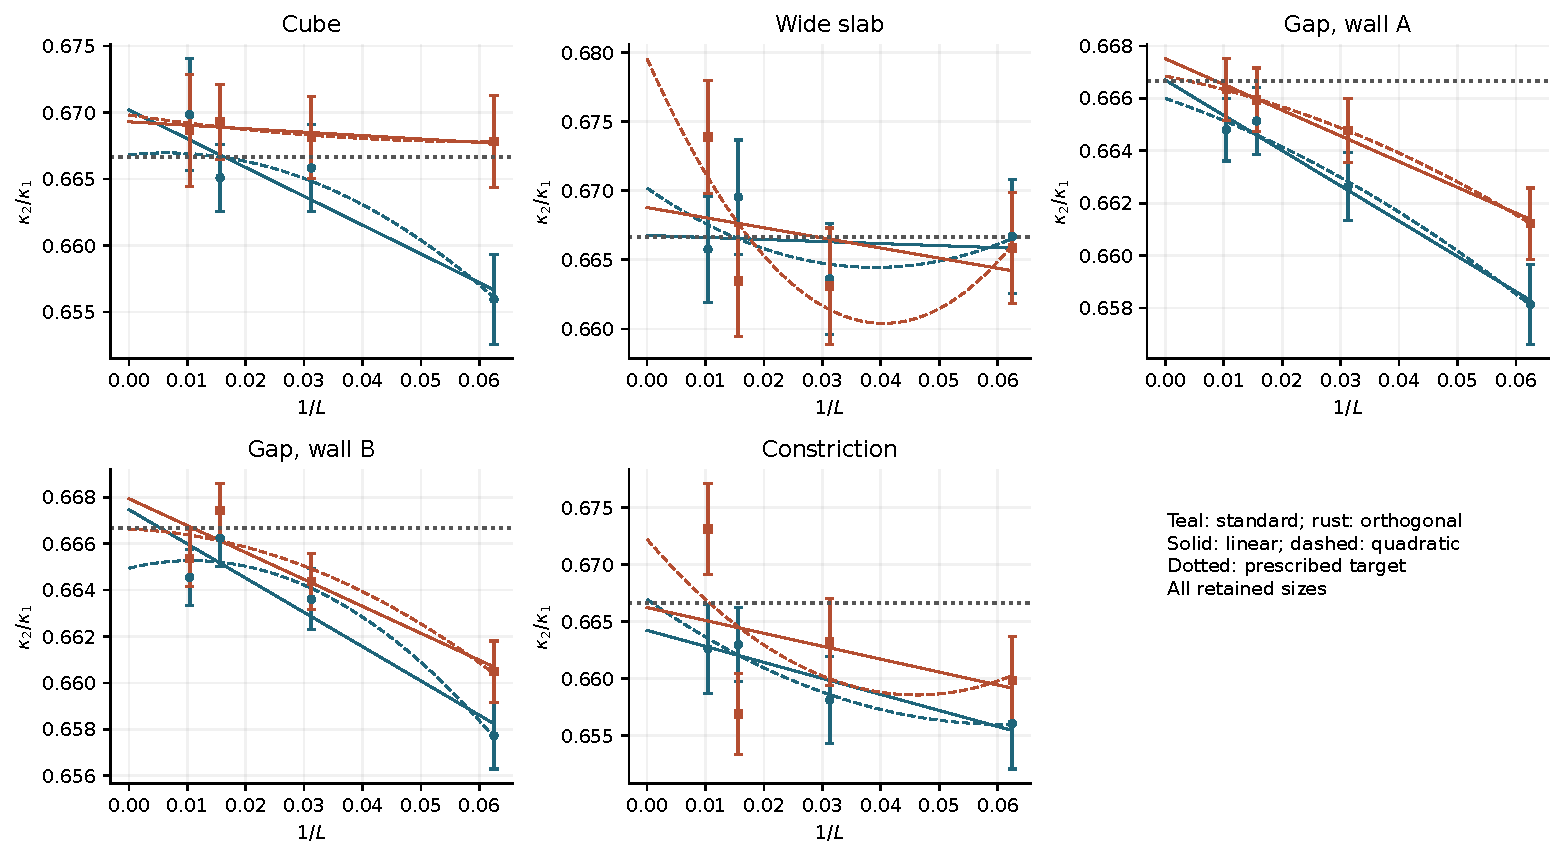
\includegraphics[width=\textwidth]{figures/original_r2.pdf}
\caption{Original second-cumulant ratios. All original sizes, both rules and both prescribed forms are shown, including the constriction's failed fit criterion.}\end{figure}
\begin{figure}[p]\centering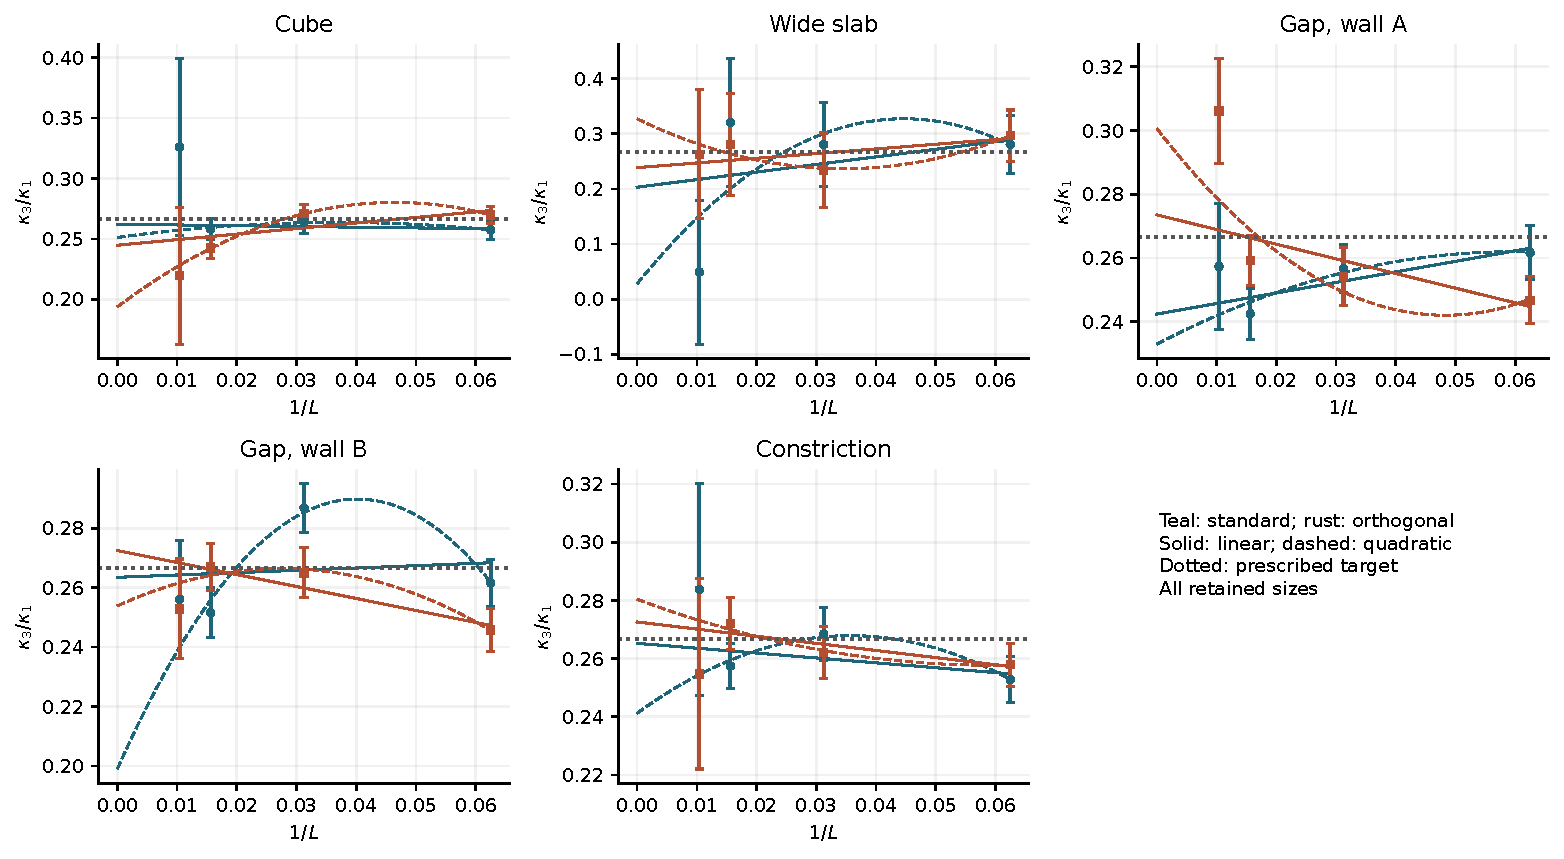
\includegraphics[width=\textwidth]{figures/original_r3.pdf}
\caption{Original third-cumulant ratios after the fixed addition where planned. The wide slab remains underpowered, and wall B does not pass the fit criterion.}\end{figure}
\begin{figure}[p]\centering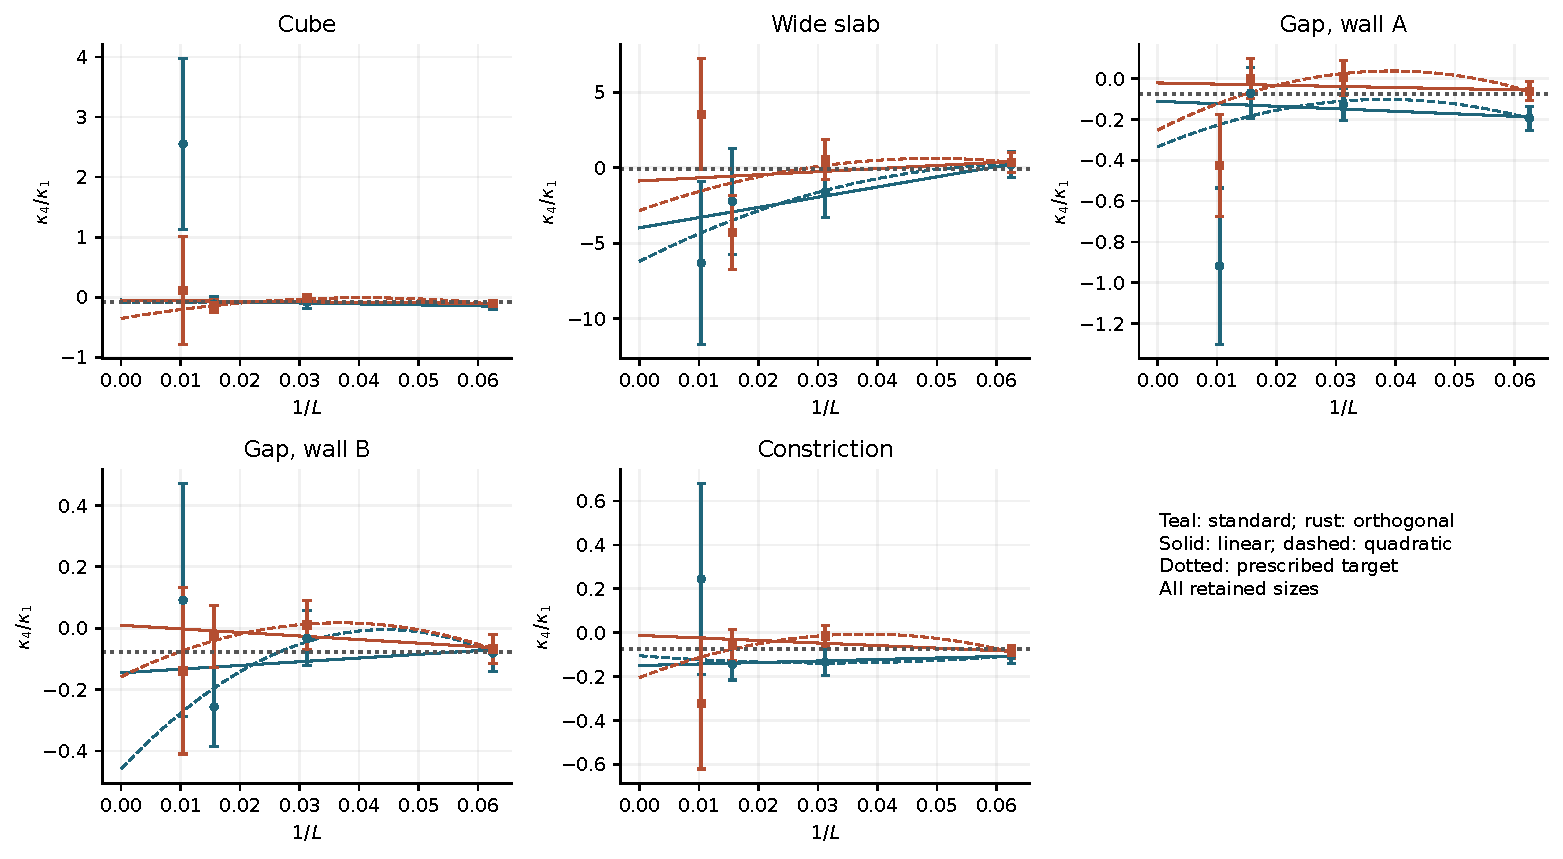
\includegraphics[width=\textwidth]{figures/original_r4.pdf}
\caption{Original fourth-cumulant ratios. No geometry supplies a conclusive fourth-cumulant decision.}\end{figure}
\begin{figure}[p]\centering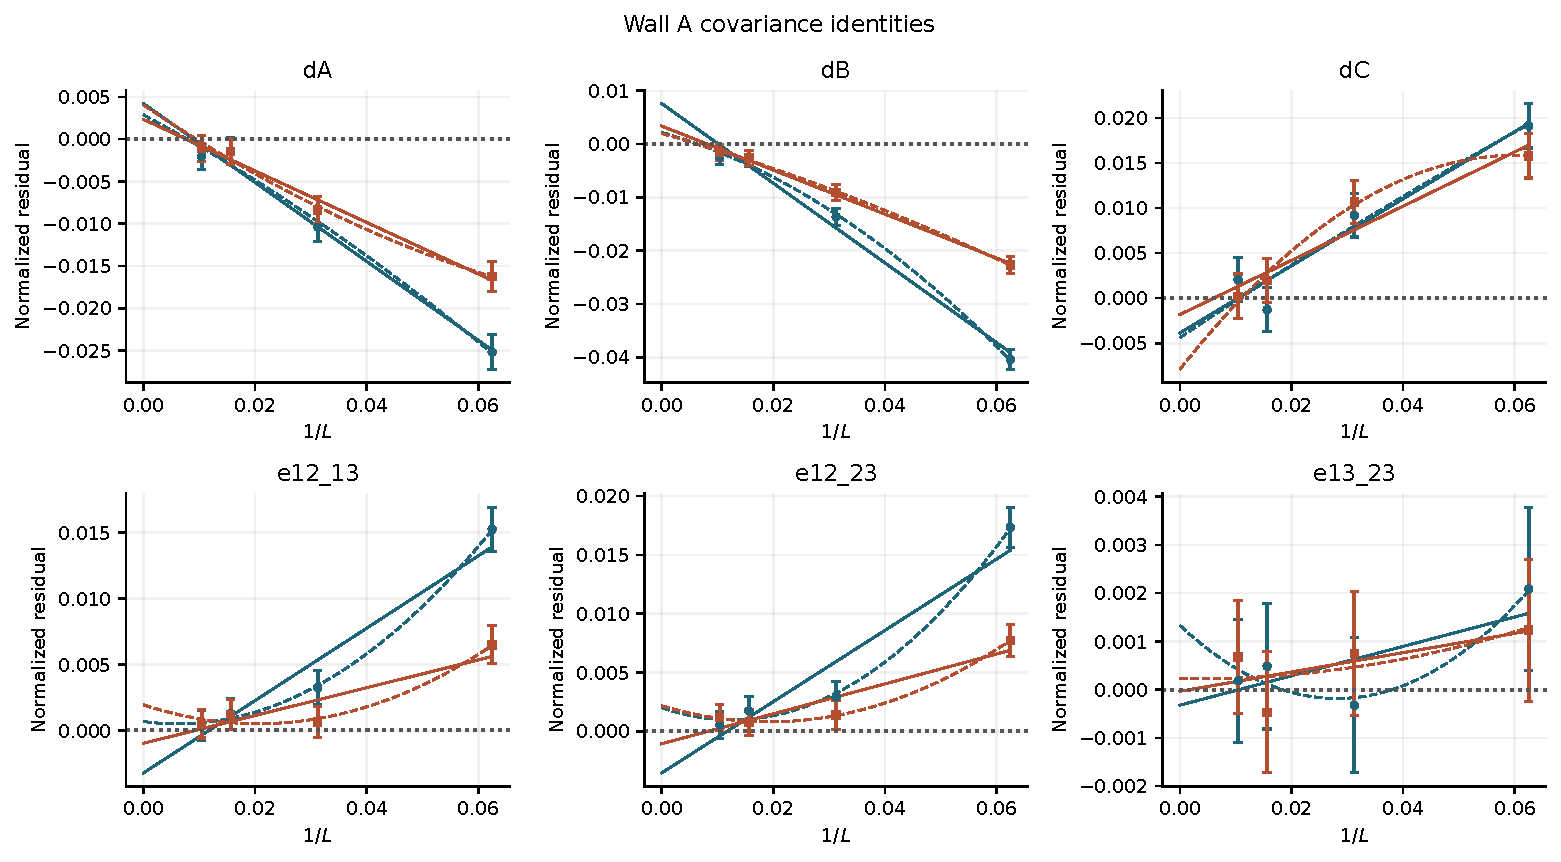
\includegraphics[width=\textwidth]{figures/identities_gap.pdf}
\caption{All six gapped-terminal identity residuals for wall A. Solid/dashed curves are linear/quadratic fits; teal/rust denote standard/orthogonal rules.}\end{figure}
\begin{figure}[p]\centering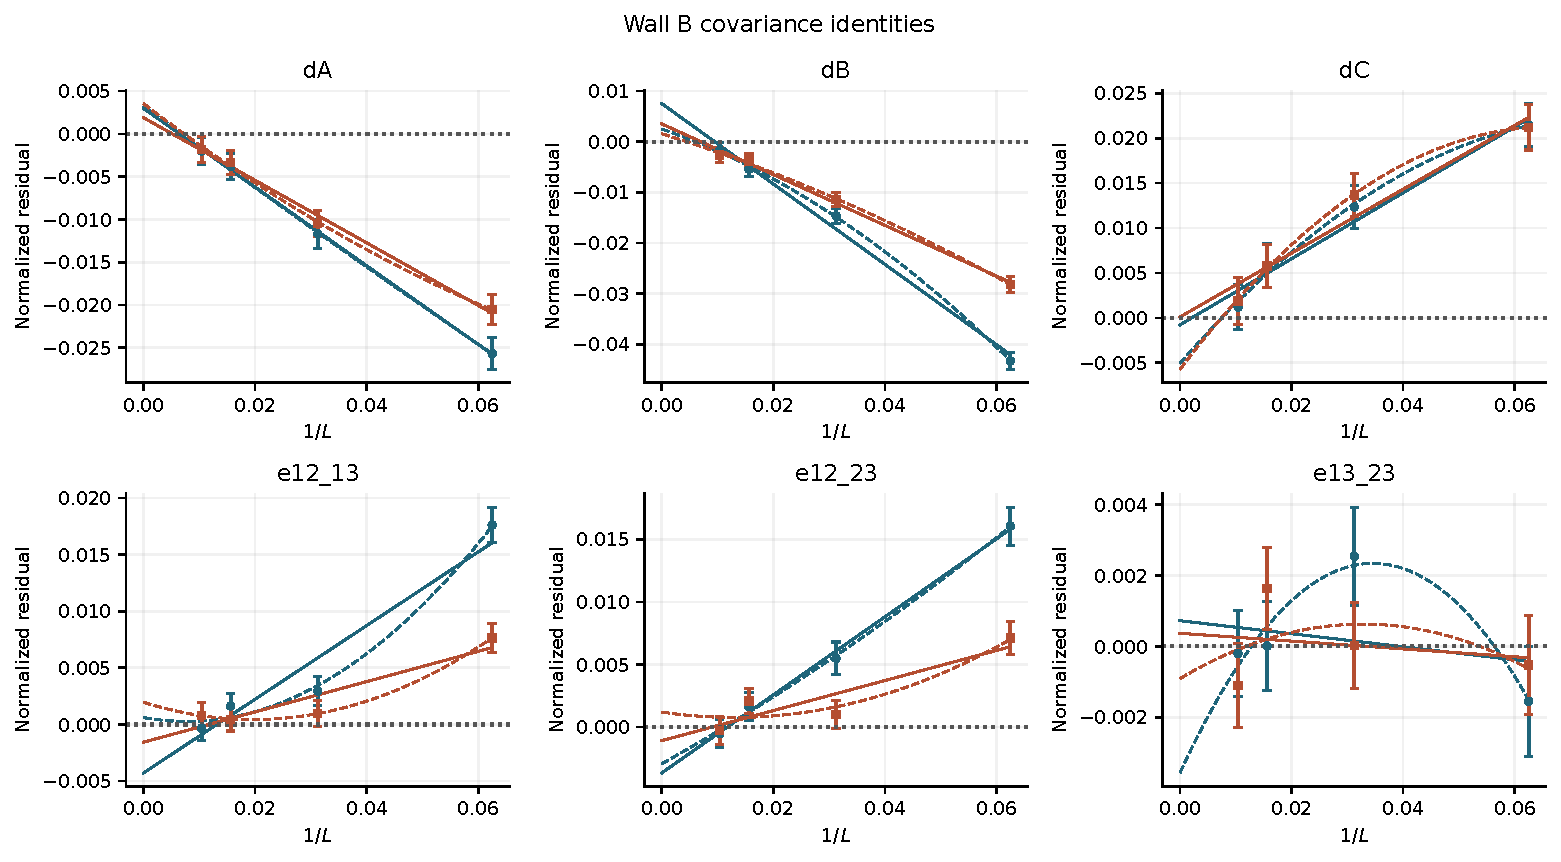
\includegraphics[width=\textwidth]{figures/identities_wall2.pdf}
\caption{The corresponding six identity residuals for wall B. Together the two walls leave five identity tests undecided.}\end{figure}
\clearpage
{\small\setlength{\tabcolsep}{3.5pt}
\begin{longtable}{lllrr}
\caption{Complete original sample allocation. The fixed addition does not change the original second-cumulant or covariance samples.}\\
\toprule
Data & Geometry & Rule & $L$ & Environments\\
\midrule
\endfirsthead
\toprule
Data & Geometry & Rule & $L$ & Environments\\
\midrule
\endhead
\bottomrule\endfoot
Initial & Cube & O & 16 & 74,000\\
Initial & Cube & O & 32 & 92,000\\
Initial & Cube & O & 64 & 108,000\\
Initial & Cube & O & 96 & 54,000\\
Initial & Cube & S & 16 & 72,000\\
Initial & Cube & S & 32 & 83,000\\
Initial & Cube & S & 64 & 142,000\\
Initial & Cube & S & 96 & 55,000\\
Initial & Gap, wall A & O & 16 & 473,000\\
Initial & Gap, wall A & O & 32 & 578,000\\
Initial & Gap, wall A & O & 64 & 603,000\\
Initial & Gap, wall A & O & 96 & 620,000\\
Initial & Gap, wall A & S & 16 & 391,000\\
Initial & Gap, wall A & S & 32 & 515,000\\
Initial & Gap, wall A & S & 64 & 555,000\\
Initial & Gap, wall A & S & 96 & 575,000\\
Initial & Constriction & O & 16 & 57,000\\
Initial & Constriction & O & 32 & 58,000\\
Initial & Constriction & O & 64 & 65,000\\
Initial & Constriction & O & 96 & 55,000\\
Initial & Constriction & S & 16 & 57,000\\
Initial & Constriction & S & 32 & 58,000\\
Initial & Constriction & S & 64 & 86,000\\
Initial & Constriction & S & 96 & 58,000\\
Initial & Wide slab & O & 16 & 54,000\\
Initial & Wide slab & O & 32 & 52,000\\
Initial & Wide slab & O & 64 & 53,000\\
Initial & Wide slab & O & 96 & 53,000\\
Initial & Wide slab & S & 16 & 52,000\\
Initial & Wide slab & S & 32 & 54,000\\
Initial & Wide slab & S & 64 & 52,000\\
Initial & Wide slab & S & 96 & 57,000\\
Initial & Gap, wall B & O & 16 & 490,000\\
Initial & Gap, wall B & O & 32 & 615,000\\
Initial & Gap, wall B & O & 64 & 673,000\\
Initial & Gap, wall B & O & 96 & 604,000\\
Initial & Gap, wall B & S & 16 & 415,000\\
Initial & Gap, wall B & S & 32 & 535,000\\
Initial & Gap, wall B & S & 64 & 603,000\\
Initial & Gap, wall B & S & 96 & 600,000\\
Fixed addition & Retroreflection & O & 16 & 218,000\\
Fixed addition & Retroreflection & O & 32 & 237,000\\
Fixed addition & Retroreflection & O & 64 & 230,000\\
Fixed addition & Retroreflection & O & 96 & 238,000\\
Fixed addition & Retroreflection & S & 16 & 212,000\\
Fixed addition & Retroreflection & S & 32 & 217,000\\
Fixed addition & Retroreflection & S & 64 & 220,000\\
Fixed addition & Retroreflection & S & 96 & 210,000\\
Fixed addition & Cube & O & 16 & 458,000\\
Fixed addition & Cube & O & 32 & 921,000\\
Fixed addition & Cube & O & 64 & 1,462,000\\
Fixed addition & Cube & S & 16 & 517,000\\
Fixed addition & Cube & S & 32 & 885,000\\
Fixed addition & Cube & S & 64 & 2,253,000\\
Fixed addition & Gap, wall A & O & 32 & 56,000\\
Fixed addition & Gap, wall A & O & 64 & 1,231,000\\
Fixed addition & Gap, wall A & S & 16 & 103,000\\
Fixed addition & Gap, wall A & S & 32 & 846,000\\
Fixed addition & Gap, wall A & S & 64 & 1,938,000\\
Fixed addition & Constriction & O & 16 & 110,000\\
Fixed addition & Constriction & O & 32 & 203,000\\
Fixed addition & Constriction & O & 64 & 426,000\\
Fixed addition & Constriction & S & 16 & 135,000\\
Fixed addition & Constriction & S & 32 & 261,000\\
Fixed addition & Constriction & S & 64 & 826,000\\
Fixed addition & Gap, wall B & O & 32 & 155,000\\
Fixed addition & Gap, wall B & O & 64 & 1,164,000\\
Fixed addition & Gap, wall B & S & 16 & 117,000\\
Fixed addition & Gap, wall B & S & 32 & 626,000\\
Fixed addition & Gap, wall B & S & 64 & 1,692,000\\
\end{longtable}}


\section{Stripe confirmation: complete reports}
The layout-difference family has four tests: zero difference and the
predicted difference, each with both forms. The family level is \(0.05\),
the fit threshold \(0.01\), the rule-agreement bound three combined standard
errors and the maximum joint standard error \(0.0075\).
The later absolute-ratio family has six tests: three masks, each with both
forms. Its corresponding precision bound is \(0.003\).
Each form has a common intercept with separate rule-dependent corrections.
Every separate-rule fit is also reported.

Raw fixed-mask ratios, the full-face ratio, the layout difference within
the absolute-data sample, higher cumulants and spectra are auxiliary where
not listed in the respective primary plan. In particular, the auxiliary
third-cumulant and spectrum diagnostics were registered during collection,
not before it, and receive no new confirmation decision.
The compact release stores every environment in both primary stripe
samples. For the later sample its columns are
\((N,2LQ_1,2LQ_2,2LQ_4,C_1,C_2,C_4)\), all exact integers.
This preserves the joint empirical distribution used by the primary
bootstrap. Full transverse marginals are needed for the auxiliary
higher-order and spectrum replay and are not included in these compact
columns. They can be regenerated from the original seeds.

{\small\setlength{\tabcolsep}{3.5pt}
\begin{longtable}{llrrr}
\caption{Stripe sample allocation and fixed bootstrap seeds. Physical seeds are recorded separately.}\\
\toprule
Data & Rule & $L$ & Environments & Bootstrap seed\\
\midrule
\endfirsthead
\toprule
Data & Rule & $L$ & Environments & Bootstrap seed\\
\midrule
\endhead
\bottomrule\endfoot
Layout & Standard & 16 & 293,000 & 330030001\\
Layout & Standard & 32 & 616,500 & 330030002\\
Layout & Standard & 64 & 251,750 & 330030003\\
Layout & Standard & 128 & 20,000 & 330030004\\
Layout & Orthogonal & 16 & 327,500 & 330030005\\
Layout & Orthogonal & 32 & 698,750 & 330030006\\
Layout & Orthogonal & 64 & 294,750 & 330030007\\
Layout & Orthogonal & 128 & 20,000 & 330030008\\
Absolute & Standard & 32 & 166,000 & 679925300\\
Absolute & Standard & 64 & 290,250 & 841496916\\
Absolute & Standard & 128 & 77,000 & 4285283429\\
Absolute & Standard & 256 & 40,000 & 1600146856\\
Absolute & Orthogonal & 32 & 166,000 & 4258797266\\
Absolute & Orthogonal & 64 & 290,250 & 2141657993\\
Absolute & Orthogonal & 128 & 77,000 & 3227410029\\
Absolute & Orthogonal & 256 & 40,000 & 1894540754\\
\end{longtable}}

{\small\setlength{\tabcolsep}{3.5pt}
\begin{longtable}{llrr}
\caption{All raw primary probabilities and Holm rejections for the two independent stripe families.}\\
\toprule
Family & Test & $p$ & Rejected\\
\midrule
\endfirsthead
\toprule
Family & Test & $p$ & Rejected\\
\midrule
\endhead
\bottomrule\endfoot
Layout & zero\_1 & 7.23e-37 & yes\\
Layout & theory\_1 & 0.543 & no\\
Layout & zero\_2 & 2.33e-06 & yes\\
Layout & theory\_2 & 0.957 & no\\
Absolute & r1\_1 & 0.762 & no\\
Absolute & r1\_2 & 0.319 & no\\
Absolute & r2\_1 & 0.528 & no\\
Absolute & r2\_2 & 0.146 & no\\
Absolute & r4\_1 & 0.381 & no\\
Absolute & r4\_2 & 0.0589 & no\\
\end{longtable}}

{\small\setlength{\tabcolsep}{3.5pt}
\begin{longtable}{lrrrr}
\caption{All absolute-data fits, including full-face, raw fixed-mask and contrast diagnostics. The three symmetry-averaged stripe ratios alone belong to the primary family.}\\
\toprule
Rule & Quantity & Degree & Intercept & $p_{\rm fit}$\\
\midrule
\endfirsthead
\toprule
Rule & Quantity & Degree & Intercept & $p_{\rm fit}$\\
\midrule
\endhead
\bottomrule\endfoot
S & rN & 1 & $0.665906\pm0.002788$ & 0.232\\
S & rN & 2 & $0.663579\pm0.005929$ & 0.0987\\
S & r1 & 1 & $0.800636\pm0.001598$ & 0.605\\
S & r1 & 2 & $0.799705\pm0.003417$ & 0.341\\
S & r2 & 1 & $0.816910\pm0.001632$ & 0.072\\
S & r2 & 2 & $0.812558\pm0.003494$ & 0.0716\\
S & r4 & 1 & $0.826134\pm0.001635$ & 0.158\\
S & r4 & 2 & $0.821426\pm0.003508$ & 0.255\\
S & raw1 & 1 & $0.799957\pm0.003422$ & 0.831\\
S & raw1 & 2 & $0.798515\pm0.007165$ & 0.573\\
S & raw2 & 1 & $0.814736\pm0.003422$ & 0.123\\
S & raw2 & 2 & $0.801480\pm0.007376$ & 0.969\\
S & raw4 & 1 & $0.823500\pm0.003396$ & 0.608\\
S & raw4 & 2 & $0.817844\pm0.007452$ & 0.619\\
S & delta41 & 1 & $0.025500\pm0.001181$ & 0.205\\
S & delta41 & 2 & $0.021746\pm0.002424$ & 0.769\\
O & rN & 1 & $0.665209\pm0.002764$ & 0.163\\
O & rN & 2 & $0.655500\pm0.005913$ & 0.612\\
O & r1 & 1 & $0.798848\pm0.001592$ & 0.3\\
O & r1 & 2 & $0.794292\pm0.003409$ & 0.735\\
O & r2 & 1 & $0.817260\pm0.001609$ & 0.361\\
O & r2 & 2 & $0.813192\pm0.003455$ & 0.587\\
O & r4 & 1 & $0.825585\pm0.001628$ & 0.0772\\
O & r4 & 2 & $0.818978\pm0.003458$ & 0.472\\
O & raw1 & 1 & $0.798301\pm0.003280$ & 0.218\\
O & raw1 & 2 & $0.791874\pm0.007167$ & 0.155\\
O & raw2 & 1 & $0.819102\pm0.003537$ & 0.671\\
O & raw2 & 2 & $0.813257\pm0.007355$ & 0.929\\
O & raw4 & 1 & $0.825974\pm0.003384$ & 0.255\\
O & raw4 & 2 & $0.815976\pm0.007290$ & 0.548\\
O & delta41 & 1 & $0.026691\pm0.001174$ & 0.209\\
O & delta41 & 2 & $0.024545\pm0.002521$ & 0.139\\
J & rN & 1 & $0.665560\pm0.001945$ & 0.253\\
J & rN & 2 & $0.659580\pm0.004139$ & 0.272\\
J & r1 & 1 & $0.799752\pm0.001116$ & 0.545\\
J & r1 & 2 & $0.797022\pm0.002399$ & 0.514\\
J & r2 & 1 & $0.817086\pm0.001130$ & 0.198\\
J & r2 & 2 & $0.812874\pm0.002408$ & 0.314\\
J & r4 & 1 & $0.825861\pm0.001150$ & 0.114\\
J & r4 & 2 & $0.820215\pm0.002456$ & 0.559\\
J & raw1 & 1 & $0.799132\pm0.002388$ & 0.618\\
J & raw1 & 2 & $0.795211\pm0.005087$ & 0.429\\
J & raw2 & 1 & $0.816903\pm0.002423$ & 0.327\\
J & raw2 & 2 & $0.807288\pm0.005145$ & 0.733\\
J & raw4 & 1 & $0.824742\pm0.002427$ & 0.552\\
J & raw4 & 2 & $0.816904\pm0.005223$ & 0.887\\
J & delta41 & 1 & $0.026081\pm0.000827$ & 0.235\\
J & delta41 & 2 & $0.023103\pm0.001750$ & 0.405\\
\end{longtable}}

{\small\setlength{\tabcolsep}{3.5pt}
\begin{longtable}{lrrrr}
\caption{All layout-data fits. Absolute ratios are secondary diagnostics; the paired difference is primary.}\\
\toprule
Rule & Quantity & Degree & Intercept & $p_{\rm fit}$\\
\midrule
\endfirsthead
\toprule
Rule & Quantity & Degree & Intercept & $p_{\rm fit}$\\
\midrule
\endhead
\bottomrule\endfoot
S & rN & 1 & $0.668690\pm0.002013$ & 0.621\\
S & rN & 2 & $0.671930\pm0.005149$ & 0.49\\
S & r1 & 1 & $0.807745\pm0.002424$ & 0.374\\
S & r1 & 2 & $0.802115\pm0.005792$ & 0.35\\
S & r2 & 1 & $0.822256\pm0.002470$ & 0.582\\
S & r2 & 2 & $0.822334\pm0.006252$ & 0.298\\
S & r4 & 1 & $0.831697\pm0.002369$ & 0.652\\
S & r4 & 2 & $0.826867\pm0.006135$ & 0.759\\
S & delta41 & 1 & $0.023946\pm0.003126$ & 0.89\\
S & delta41 & 2 & $0.024733\pm0.007817$ & 0.638\\
O & rN & 1 & $0.664260\pm0.001875$ & 0.643\\
O & rN & 2 & $0.668104\pm0.004524$ & 0.824\\
O & r1 & 1 & $0.799584\pm0.002178$ & 0.853\\
O & r1 & 2 & $0.796940\pm0.005645$ & 0.826\\
O & r2 & 1 & $0.818948\pm0.002270$ & 0.909\\
O & r2 & 2 & $0.820895\pm0.005799$ & 0.819\\
O & r4 & 1 & $0.828765\pm0.002302$ & 0.424\\
O & r4 & 2 & $0.822528\pm0.005842$ & 0.555\\
O & delta41 & 1 & $0.029144\pm0.002854$ & 0.711\\
O & delta41 & 2 & $0.025521\pm0.007349$ & 0.531\\
J & $\Delta v$ & 1 & $0.026719\pm0.002106$ & 0.791\\
J & $\Delta v$ & 2 & $0.025149\pm0.005325$ & 0.892\\
\end{longtable}}


\section{Retrospective comparisons and unfavorable diagnostics}
The older standard-rule data show a common linear offset of
\(0.0070564322\pm0.0016158417\) in the three absolute stripe ratios.
Their covariance-aware shape test after removing a common offset has
\(p=0.7386\). This distinguishes a layout contrast from an absolute test;
it does not justify removing the offset from confirmation data.
All-size pooled fits below retain this upward linear tendency, including
\(L=16\); the quadratic fits and fresh larger-size sample behave differently.
Curvature is a possible explanation only.

{\small\setlength{\tabcolsep}{3.5pt}
\begin{longtable}{lrrrrr}
\caption{All retrospective all-size pooled fits. Fixed uses fixed-mask estimators in both batches; Mixed uses orbit averaging for the later batch. Neither changes a primary analysis.}\\
\toprule
Method & Rule & Quantity & Degree & Intercept & $p_{\rm fit}$\\
\midrule
\endfirsthead
\toprule
Method & Rule & Quantity & Degree & Intercept & $p_{\rm fit}$\\
\midrule
\endhead
\bottomrule\endfoot
Fixed & S & r1 & 1 & $0.805533\pm0.001741$ & 0.409\\
Fixed & S & r1 & 2 & $0.799387\pm0.003393$ & 0.902\\
Fixed & S & r2 & 1 & $0.820625\pm0.001749$ & 0.152\\
Fixed & S & r2 & 2 & $0.815686\pm0.003489$ & 0.245\\
Fixed & S & r4 & 1 & $0.829422\pm0.001719$ & 0.437\\
Fixed & S & r4 & 2 & $0.823008\pm0.003361$ & 0.937\\
Fixed & O & r1 & 1 & $0.799968\pm0.001622$ & 0.633\\
Fixed & O & r1 & 2 & $0.797655\pm0.003299$ & 0.599\\
Fixed & O & r2 & 1 & $0.819273\pm0.001689$ & 0.982\\
Fixed & O & r2 & 2 & $0.819692\pm0.003402$ & 0.956\\
Fixed & O & r4 & 1 & $0.827269\pm0.001663$ & 0.492\\
Fixed & O & r4 & 2 & $0.823076\pm0.003328$ & 0.64\\
Fixed & J & r1 & 1 & $0.802640\pm0.001182$ & 0.253\\
Fixed & J & r1 & 2 & $0.798505\pm0.002382$ & 0.91\\
Fixed & J & r2 & 1 & $0.819917\pm0.001193$ & 0.627\\
Fixed & J & r2 & 2 & $0.817740\pm0.002393$ & 0.673\\
Fixed & J & r4 & 1 & $0.828301\pm0.001218$ & 0.522\\
Fixed & J & r4 & 2 & $0.823042\pm0.002337$ & 0.946\\
Mixed & S & r1 & 1 & $0.803204\pm0.001119$ & 0.153\\
Mixed & S & r1 & 2 & $0.799128\pm0.001948$ & 0.747\\
Mixed & S & r2 & 1 & $0.818771\pm0.001118$ & 0.138\\
Mixed & S & r2 & 2 & $0.815967\pm0.002024$ & 0.243\\
Mixed & S & r4 & 1 & $0.828672\pm0.001107$ & 0.156\\
Mixed & S & r4 & 2 & $0.824458\pm0.001983$ & 0.765\\
Mixed & O & r1 & 1 & $0.800309\pm0.001082$ & 0.446\\
Mixed & O & r1 & 2 & $0.797970\pm0.001906$ & 0.606\\
Mixed & O & r2 & 1 & $0.818049\pm0.001122$ & 0.847\\
Mixed & O & r2 & 2 & $0.817015\pm0.001923$ & 0.811\\
Mixed & O & r4 & 1 & $0.827050\pm0.001118$ & 0.211\\
Mixed & O & r4 & 2 & $0.823700\pm0.001930$ & 0.529\\
Mixed & J & r1 & 1 & $0.801727\pm0.000769$ & 0.137\\
Mixed & J & r1 & 2 & $0.798547\pm0.001343$ & 0.839\\
Mixed & J & r2 & 1 & $0.818399\pm0.000781$ & 0.48\\
Mixed & J & r2 & 2 & $0.816501\pm0.001370$ & 0.61\\
Mixed & J & r4 & 1 & $0.827847\pm0.000800$ & 0.131\\
Mixed & J & r4 & 2 & $0.824077\pm0.001366$ & 0.816\\
\end{longtable}}

{\small\setlength{\tabcolsep}{3.5pt}
\begin{longtable}{lrrrr}
\caption{All retrospective reconstructed full-face and difference statistics. They reuse the original retroreflecting environments.}\\
\toprule
Rule & Quantity & Degree & Intercept & $p_{\rm fit}$\\
\midrule
\endfirsthead
\toprule
Rule & Quantity & Degree & Intercept & $p_{\rm fit}$\\
\midrule
\endhead
\bottomrule\endfoot
S & r\_N & 1 & $0.668901\pm0.001808$ & 0.68\\
S & r\_N & 2 & $0.670848\pm0.004054$ & 0.488\\
S & r\_D & 1 & $0.973271\pm0.002694$ & 0.0467\\
S & r\_D & 2 & $0.971685\pm0.005835$ & 0.014\\
S & cov\_CF\_over\_N & 1 & $-0.076087\pm0.000811$ & 0.0462\\
S & cov\_CF\_over\_N & 2 & $-0.075181\pm0.001785$ & 0.0158\\
S & mean\_imbalance & 1 & $-0.000008\pm0.000203$ & 0.822\\
S & mean\_imbalance & 2 & $0.000083\pm0.000455$ & 0.559\\
O & r\_N & 1 & $0.667421\pm0.001668$ & 0.0378\\
O & r\_N & 2 & $0.666500\pm0.003793$ & 0.0109\\
O & r\_D & 1 & $0.968273\pm0.002474$ & 0.286\\
O & r\_D & 2 & $0.963771\pm0.005622$ & 0.194\\
O & cov\_CF\_over\_N & 1 & $-0.075202\pm0.000749$ & 0.0361\\
O & cov\_CF\_over\_N & 2 & $-0.074333\pm0.001678$ & 0.012\\
O & mean\_imbalance & 1 & $0.000074\pm0.000230$ & 0.926\\
O & mean\_imbalance & 2 & $0.000230\pm0.000504$ & 0.851\\
\end{longtable}}

The reconstructed full-face count in the retroreflecting environments
uses \(N=C+f_L\) and no additional sample. The partial-port comparison
is retrospective because it followed the original rejection of \(2/3\).
It is not counted as an additional independent confirmation of the stripe law.

\section{Exploratory geometries, third cumulants and spectrum}
The diagnostic collection consists of 128,000 calibration environments and
68,000 subsequently held-out environments, for a total of 196,000.
The latter were new when the fixed local-response prediction was tested;
all later combined and source-matching uses are retrospective.
Both rules and all sizes \(16,32,64,128,256\) are retained.
The quarter-strip and square absolute ratios are about \(0.5\%\) high.
Their difference is closer to the geometric target. Neither fact establishes
an asymptotic conclusion for \(p=1/4\).

The fresh half-open and independent diagnostic single-stripe third-cumulant
estimates lie on opposite sides of the saddle value. The samples cover
different sizes; their linear discrepancy is about two combined standard
errors. Masks share environments and a full-face third-cumulant contribution,
so agreement among masks is correlated evidence.

\begin{figure}[htbp]\centering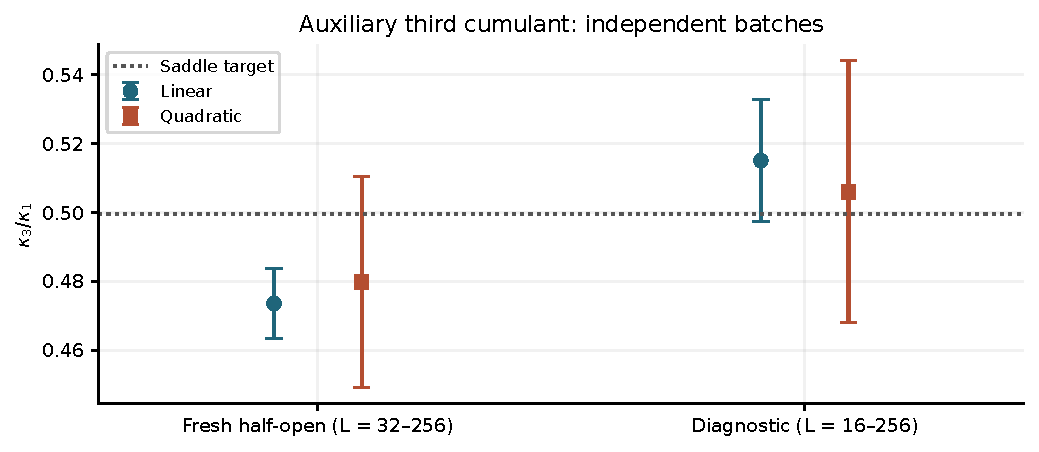
\includegraphics[width=.85\textwidth]{figures/third_batches.pdf}
\caption{Auxiliary third-cumulant estimates from two independent collections, with both extrapolations and one-standard-error bars.}\end{figure}
{\small\setlength{\tabcolsep}{3.5pt}
\begin{longtable}{lrrrrr}
\caption{All auxiliary third-cumulant fits for the fresh half-open data, with refined deterministic targets.}\\
\toprule
Rule & Quantity & Degree & Target & Intercept & $p_{\rm fit}$\\
\midrule
\endfirsthead
\toprule
Rule & Quantity & Degree & Target & Intercept & $p_{\rm fit}$\\
\midrule
\endhead
\bottomrule\endfoot
S & h1 & 1 & 0.499442417 & $0.472570\pm0.016065$ & 0.357\\
S & h1 & 2 & 0.499442417 & $0.505052\pm0.048637$ & 0.209\\
S & h2 & 1 & 0.532821444 & $0.509247\pm0.016054$ & 0.857\\
S & h2 & 2 & 0.532821444 & $0.483424\pm0.048867$ & 0.921\\
S & h4 & 1 & 0.549715205 & $0.525261\pm0.016054$ & 0.728\\
S & h4 & 2 & 0.549715205 & $0.510619\pm0.049387$ & 0.463\\
S & hN & 1 & 0.266666667 & $0.189273\pm0.044674$ & 0.691\\
S & hN & 2 & 0.266666667 & $0.211106\pm0.136632$ & 0.399\\
O & h1 & 1 & 0.499442417 & $0.474267\pm0.013113$ & 0.938\\
O & h1 & 2 & 0.499442417 & $0.463725\pm0.039239$ & 0.83\\
O & h2 & 1 & 0.532821444 & $0.525337\pm0.013268$ & 0.692\\
O & h2 & 2 & 0.532821444 & $0.541223\pm0.040942$ & 0.451\\
O & h4 & 1 & 0.549715205 & $0.544327\pm0.013926$ & 0.866\\
O & h4 & 2 & 0.549715205 & $0.549277\pm0.041379$ & 0.601\\
O & hN & 1 & 0.266666667 & $0.237602\pm0.036399$ & 0.874\\
O & hN & 2 & 0.266666667 & $0.191800\pm0.111056$ & 0.781\\
J & h1 & 1 & 0.499442417 & $0.473576\pm0.010200$ & 0.822\\
J & h1 & 2 & 0.499442417 & $0.479796\pm0.030581$ & 0.562\\
J & h2 & 1 & 0.532821444 & $0.518688\pm0.010289$ & 0.899\\
J & h2 & 2 & 0.532821444 & $0.517985\pm0.031434$ & 0.711\\
J & h4 & 1 & 0.549715205 & $0.536241\pm0.010581$ & 0.888\\
J & h4 & 2 & 0.549715205 & $0.533323\pm0.031591$ & 0.762\\
J & hN & 1 & 0.266666667 & $0.218150\pm0.027801$ & 0.89\\
J & hN & 2 & 0.266666667 & $0.199247\pm0.085880$ & 0.849\\
\end{longtable}}

{\small\setlength{\tabcolsep}{3.5pt}
\begin{longtable}{lllrrr}
\caption{All exploratory diagnostic fits, including both batches separately and together, both rules and descriptive joint fits. No additional confirmation decision is made.}\\
\toprule
Data & Rule & Observable & Degree & Intercept & $p_{\rm fit}$\\
\midrule
\endfirsthead
\toprule
Data & Rule & Observable & Degree & Intercept & $p_{\rm fit}$\\
\midrule
\endhead
\bottomrule\endfoot
Calibration & S & $v_N$ & 1 & $0.673969\pm0.006996$ & 0.619\\
Calibration & S & $v_N$ & 2 & $0.666737\pm0.012266$ & 0.53\\
Calibration & S & $h_N$ & 1 & $0.421095\pm0.099658$ & 0.662\\
Calibration & S & $h_N$ & 2 & $0.206083\pm0.223955$ & 0.804\\
Calibration & S & $v_{1/2,1}$ & 1 & $0.803660\pm0.004009$ & 0.666\\
Calibration & S & $v_{1/2,1}$ & 2 & $0.796983\pm0.007006$ & 0.895\\
Calibration & S & Quarter strip & 1 & $0.879956\pm0.002807$ & 0.217\\
Calibration & S & Quarter strip & 2 & $0.871540\pm0.004885$ & 0.992\\
Calibration & S & Square & 1 & $0.875283\pm0.002744$ & 0.424\\
Calibration & S & Square & 2 & $0.869409\pm0.004774$ & 0.765\\
Calibration & S & $h_{1/2,1}$ & 1 & $0.585006\pm0.036161$ & 0.748\\
Calibration & S & $h_{1/2,1}$ & 2 & $0.577605\pm0.080579$ & 0.546\\
Calibration & S & Square minus strip & 1 & $-0.004634\pm0.001305$ & 0.266\\
Calibration & S & Square minus strip & 2 & $-0.002137\pm0.002272$ & 0.341\\
Calibration & O & $v_N$ & 1 & $0.661504\pm0.006960$ & 0.454\\
Calibration & O & $v_N$ & 2 & $0.663135\pm0.012339$ & 0.273\\
Calibration & O & $h_N$ & 1 & $0.185978\pm0.078446$ & 0.101\\
Calibration & O & $h_N$ & 2 & $-0.180217\pm0.184878$ & 0.483\\
Calibration & O & $v_{1/2,1}$ & 1 & $0.799435\pm0.003975$ & 0.449\\
Calibration & O & $v_{1/2,1}$ & 2 & $0.804737\pm0.007010$ & 0.406\\
Calibration & O & Quarter strip & 1 & $0.877267\pm0.002794$ & 0.217\\
Calibration & O & Quarter strip & 2 & $0.882834\pm0.004903$ & 0.282\\
Calibration & O & Square & 1 & $0.874590\pm0.002735$ & 0.562\\
Calibration & O & Square & 2 & $0.878548\pm0.004797$ & 0.594\\
Calibration & O & $h_{1/2,1}$ & 1 & $0.464553\pm0.028497$ & 0.697\\
Calibration & O & $h_{1/2,1}$ & 2 & $0.436471\pm0.064514$ & 0.549\\
Calibration & O & Square minus strip & 1 & $-0.002676\pm0.001315$ & 0.5\\
Calibration & O & Square minus strip & 2 & $-0.004226\pm0.002291$ & 0.432\\
Calibration & J & $v_N$ & 1 & $0.667705\pm0.004934$ & 0.54\\
Calibration & J & $v_N$ & 2 & $0.664947\pm0.008699$ & 0.563\\
Calibration & J & $h_N$ & 1 & $0.275925\pm0.061641$ & 0.128\\
Calibration & J & $h_N$ & 2 & $-0.023656\pm0.142574$ & 0.599\\
Calibration & J & $v_{1/2,1}$ & 1 & $0.801530\pm0.002822$ & 0.687\\
Calibration & J & $v_{1/2,1}$ & 2 & $0.800858\pm0.004955$ & 0.756\\
Calibration & J & Quarter strip & 1 & $0.878606\pm0.001980$ & 0.228\\
Calibration & J & Quarter strip & 2 & $0.877166\pm0.003460$ & 0.39\\
Calibration & J & Square & 1 & $0.874935\pm0.001937$ & 0.675\\
Calibration & J & Square & 2 & $0.873957\pm0.003384$ & 0.638\\
Calibration & J & $h_{1/2,1}$ & 1 & $0.510701\pm0.022382$ & 0.219\\
Calibration & J & $h_{1/2,1}$ & 2 & $0.491601\pm0.050362$ & 0.51\\
Calibration & J & Square minus strip & 1 & $-0.003663\pm0.000926$ & 0.385\\
Calibration & J & Square minus strip & 2 & $-0.003173\pm0.001613$ & 0.514\\
Held-out & S & $v_N$ & 1 & $0.661996\pm0.008225$ & 0.349\\
Held-out & S & $v_N$ & 2 & $0.664418\pm0.013435$ & 0.198\\
Held-out & S & $h_N$ & 1 & $0.220628\pm0.124529$ & 0.133\\
Held-out & S & $h_N$ & 2 & $0.367875\pm0.253102$ & 0.0763\\
Held-out & S & $v_{1/2,1}$ & 1 & $0.804928\pm0.004750$ & 0.438\\
Held-out & S & $v_{1/2,1}$ & 2 & $0.813086\pm0.007785$ & 0.618\\
Held-out & S & Quarter strip & 1 & $0.880615\pm0.003370$ & 0.52\\
Held-out & S & Quarter strip & 2 & $0.887197\pm0.005539$ & 0.991\\
Held-out & S & Square & 1 & $0.879844\pm0.003304$ & 0.421\\
Held-out & S & Square & 2 & $0.886469\pm0.005448$ & 0.787\\
Held-out & S & $h_{1/2,1}$ & 1 & $0.476540\pm0.044044$ & 0.867\\
Held-out & S & $h_{1/2,1}$ & 2 & $0.496274\pm0.090781$ & 0.717\\
Held-out & S & Square minus strip & 1 & $-0.000774\pm0.001570$ & 0.584\\
Held-out & S & Square minus strip & 2 & $-0.000889\pm0.002559$ & 0.378\\
Held-out & O & $v_N$ & 1 & $0.663257\pm0.008260$ & 0.249\\
Held-out & O & $v_N$ & 2 & $0.676727\pm0.013521$ & 0.282\\
Held-out & O & $h_N$ & 1 & $0.287197\pm0.105017$ & 0.598\\
Held-out & O & $h_N$ & 2 & $0.264273\pm0.211424$ & 0.394\\
Held-out & O & $v_{1/2,1}$ & 1 & $0.800744\pm0.004751$ & 0.352\\
Held-out & O & $v_{1/2,1}$ & 2 & $0.802077\pm0.007785$ & 0.2\\
Held-out & O & Quarter strip & 1 & $0.878155\pm0.003368$ & 0.4\\
Held-out & O & Quarter strip & 2 & $0.875162\pm0.005525$ & 0.289\\
Held-out & O & Square & 1 & $0.875503\pm0.003279$ & 0.249\\
Held-out & O & Square & 2 & $0.871111\pm0.005392$ & 0.216\\
Held-out & O & $h_{1/2,1}$ & 1 & $0.544151\pm0.037747$ & 0.732\\
Held-out & O & $h_{1/2,1}$ & 2 & $0.533293\pm0.075626$ & 0.532\\
Held-out & O & Square minus strip & 1 & $-0.002674\pm0.001570$ & 0.885\\
Held-out & O & Square minus strip & 2 & $-0.004047\pm0.002558$ & 0.91\\
Held-out & J & $v_N$ & 1 & $0.662624\pm0.005828$ & 0.387\\
Held-out & J & $v_N$ & 2 & $0.670534\pm0.009530$ & 0.288\\
Held-out & J & $h_N$ & 1 & $0.259531\pm0.080281$ & 0.366\\
Held-out & J & $h_N$ & 2 & $0.306852\pm0.162261$ & 0.213\\
Held-out & J & $v_{1/2,1}$ & 1 & $0.802837\pm0.003359$ & 0.498\\
Held-out & J & $v_{1/2,1}$ & 2 & $0.807581\pm0.005505$ & 0.394\\
Held-out & J & Quarter strip & 1 & $0.879385\pm0.002382$ & 0.602\\
Held-out & J & Quarter strip & 2 & $0.881165\pm0.003912$ & 0.432\\
Held-out & J & Square & 1 & $0.877657\pm0.002328$ & 0.35\\
Held-out & J & Square & 2 & $0.878710\pm0.003833$ & 0.182\\
Held-out & J & $h_{1/2,1}$ & 1 & $0.515520\pm0.028661$ & 0.848\\
Held-out & J & $h_{1/2,1}$ & 2 & $0.518127\pm0.058105$ & 0.846\\
Held-out & J & Square minus strip & 1 & $-0.001724\pm0.001110$ & 0.853\\
Held-out & J & Square minus strip & 2 & $-0.002469\pm0.001809$ & 0.716\\
Combined & S & $v_N$ & 1 & $0.668692\pm0.005310$ & 0.706\\
Combined & S & $v_N$ & 2 & $0.664796\pm0.009041$ & 0.572\\
Combined & S & $h_N$ & 1 & $0.339106\pm0.077755$ & 0.265\\
Combined & S & $h_N$ & 2 & $0.250579\pm0.167732$ & 0.164\\
Combined & S & $v_{1/2,1}$ & 1 & $0.804012\pm0.003053$ & 0.968\\
Combined & S & $v_{1/2,1}$ & 2 & $0.803617\pm0.005197$ & 0.883\\
Combined & S & Quarter strip & 1 & $0.880268\pm0.002149$ & 0.883\\
Combined & S & Quarter strip & 2 & $0.878029\pm0.003656$ & 0.958\\
Combined & S & Square & 1 & $0.877076\pm0.002104$ & 0.929\\
Combined & S & Square & 2 & $0.876735\pm0.003585$ & 0.802\\
Combined & S & $h_{1/2,1}$ & 1 & $0.543120\pm0.027936$ & 0.893\\
Combined & S & $h_{1/2,1}$ & 2 & $0.537200\pm0.060256$ & 0.74\\
Combined & S & Square minus strip & 1 & $-0.003181\pm0.001000$ & 0.158\\
Combined & S & Square minus strip & 2 & $-0.001381\pm0.001695$ & 0.176\\
Combined & O & $v_N$ & 1 & $0.662343\pm0.005308$ & 0.117\\
Combined & O & $v_N$ & 2 & $0.668798\pm0.009093$ & 0.0773\\
Combined & O & $h_N$ & 1 & $0.223005\pm0.063110$ & 0.485\\
Combined & O & $h_N$ & 2 & $0.031525\pm0.139835$ & 0.955\\
Combined & O & $v_{1/2,1}$ & 1 & $0.800010\pm0.003040$ & 0.14\\
Combined & O & $v_{1/2,1}$ & 2 & $0.803666\pm0.005194$ & 0.0941\\
Combined & O & Quarter strip & 1 & $0.877589\pm0.002144$ & 0.147\\
Combined & O & Quarter strip & 2 & $0.879681\pm0.003657$ & 0.0879\\
Combined & O & Square & 1 & $0.874959\pm0.002094$ & 0.303\\
Combined & O & Square & 2 & $0.875560\pm0.003573$ & 0.166\\
Combined & O & $h_{1/2,1}$ & 1 & $0.496337\pm0.022771$ & 0.767\\
Combined & O & $h_{1/2,1}$ & 2 & $0.485272\pm0.049088$ & 0.583\\
Combined & O & Square minus strip & 1 & $-0.002661\pm0.001005$ & 0.637\\
Combined & O & Square minus strip & 2 & $-0.004122\pm0.001702$ & 0.753\\
Combined & J & $v_N$ & 1 & $0.665516\pm0.003754$ & 0.333\\
Combined & J & $v_N$ & 2 & $0.666786\pm0.006411$ & 0.275\\
Combined & J & $h_N$ & 1 & $0.269114\pm0.049001$ & 0.354\\
Combined & J & $h_N$ & 2 & $0.121345\pm0.107406$ & 0.452\\
Combined & J & $v_{1/2,1}$ & 1 & $0.802002\pm0.002154$ & 0.472\\
Combined & J & $v_{1/2,1}$ & 2 & $0.803641\pm0.003674$ & 0.419\\
Combined & J & Quarter strip & 1 & $0.878925\pm0.001518$ & 0.45\\
Combined & J & Quarter strip & 2 & $0.878854\pm0.002585$ & 0.409\\
Combined & J & Square & 1 & $0.876012\pm0.001484$ & 0.708\\
Combined & J & Square & 2 & $0.876146\pm0.002530$ & 0.537\\
Combined & J & $h_{1/2,1}$ & 1 & $0.515012\pm0.017650$ & 0.841\\
Combined & J & $h_{1/2,1}$ & 2 & $0.505987\pm0.038058$ & 0.831\\
Combined & J & Square minus strip & 1 & $-0.002922\pm0.000709$ & 0.425\\
Combined & J & Square minus strip & 2 & $-0.002746\pm0.001201$ & 0.376\\
\end{longtable}}

\begin{figure}[htbp]\centering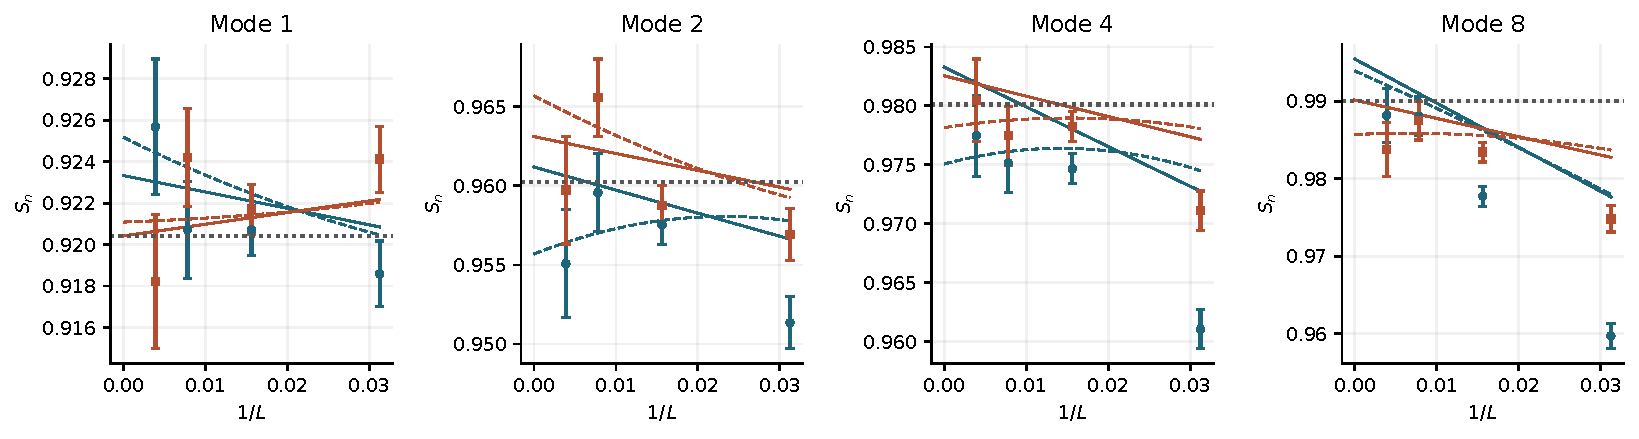
\includegraphics[width=\textwidth]{figures/spectrum.pdf}
\caption{Auxiliary transverse spectrum, all sizes and both rules. The continuum target is \(S_n=1-I(2\pi n)\). These correlated modes do not enter the primary confirmation family.}\end{figure}
{\small\setlength{\tabcolsep}{3.5pt}
\begin{longtable}{lrrrr}
\caption{All auxiliary spatial-spectrum fits. Modes share environments and are correlated.}\\
\toprule
Rule & Mode & Degree & Intercept & $p_{\rm fit}$\\
\midrule
\endfirsthead
\toprule
Rule & Mode & Degree & Intercept & $p_{\rm fit}$\\
\midrule
\endhead
\bottomrule\endfoot
S & 1 & 1 & $0.923333\pm0.001941$ & 0.549\\
S & 1 & 2 & $0.925177\pm0.004157$ & 0.331\\
S & 2 & 1 & $0.961187\pm0.002019$ & 0.229\\
S & 2 & 2 & $0.955687\pm0.004325$ & 0.35\\
S & 4 & 1 & $0.983274\pm0.002046$ & 0.0857\\
S & 4 & 2 & $0.975058\pm0.004382$ & 0.519\\
S & 8 & 1 & $0.995469\pm0.002060$ & 0.599\\
S & 8 & 2 & $0.993938\pm0.004433$ & 0.35\\
O & 1 & 1 & $0.920420\pm0.001944$ & 0.306\\
O & 1 & 2 & $0.921088\pm0.004148$ & 0.126\\
O & 2 & 1 & $0.963107\pm0.002020$ & 0.127\\
O & 2 & 2 & $0.965689\pm0.004328$ & 0.0554\\
O & 4 & 1 & $0.982540\pm0.002062$ & 0.388\\
O & 4 & 2 & $0.978145\pm0.004427$ & 0.426\\
O & 8 & 1 & $0.990160\pm0.002067$ & 0.317\\
O & 8 & 2 & $0.985719\pm0.004421$ & 0.316\\
J & 1 & 1 & $0.921879\pm0.001374$ & 0.455\\
J & 1 & 2 & $0.923128\pm0.002936$ & 0.288\\
J & 2 & 1 & $0.962147\pm0.001428$ & 0.185\\
J & 2 & 2 & $0.960684\pm0.003059$ & 0.0653\\
J & 4 & 1 & $0.982910\pm0.001452$ & 0.231\\
J & 4 & 2 & $0.976585\pm0.003114$ & 0.73\\
J & 8 & 1 & $0.992824\pm0.001459$ & 0.25\\
J & 8 & 2 & $0.989818\pm0.003130$ & 0.308\\
\end{longtable}}


\section{Why the finite-size program stopped}
Specified finite-range fourth-order response moments were calibrated on
the first diagnostic sample. The fixed range-two prediction was then
tested on the held-out sample. The four joint probabilities were approximately
\(0.303,0.288,0.620,0.612\), with no Holm rejection.
This means that these tests did not exclude that candidate response model
at their attained resolution. Coefficients depended on the chosen
subtraction and range; they were not unique microscopic couplings.
At \(L=256\), changing range from one to three changed one quarter-strip
prediction by about \(0.000674\pm0.000164\), larger than the desired
\(10^{-4}\) model-error scale.

Subsequent work measured all output separations, separated near and far
contributions with their covariance, and checked the exact cancellation
of artificial range dependence in their sum. Reconstructing a measured
window variance from the same complete measured response is an identity,
not an independent finite-parameter prediction.
Fourth- and sixth-order source matching, selected bulk, surface and
contact-line terms, and specified two-loop calculations were pursued.
The resulting seven-parameter subset was full rank, with a condition number
of order \(10^3\). It must not be described as algebraically rank deficient.
That does not establish complete physical identifiability or control of all
operators of the same order.

The resulting 264 candidate finite-size predictions had statistical
covariances but no bounded physical remainder. The corrected single-stripe
third-cumulant linear/quadratic intercepts, approximately \(0.501981\) and
\(0.499560\), did not explain the older downward estimate near \(0.474\).
Numerical mesh refinement of a continuum calculation is not physical
size refinement of the microscopic model.
The proposed subsequent confirmation was therefore never frozen or sampled.
The user stopped further research and chose a public report of the limited
results. No correction from this unfinished program is applied to the
main estimates or their uncertainties.

\section{Reproduction and evidential limits}
The \href{https://github.com/SHIN09-git/mirror3d-partial-ports/releases/tag/v1.0.0}{repository} provides a numeric source registry with JSON pointers,
file hashes, exact original seed allocations, a standalone sampler and
the original statistical cores with portable input adapters.
The verification script rebuilds all tables and figures, checks numeric
sources and repeats the closed-form calculation.
In a new Python 3.12 environment with the locked dependencies, replay of
both stripe bootstraps, both extrapolations and all associated decisions
gave zero difference from the stored outputs in 349,312 numeric comparisons.
Four original blocks, containing 4,500 environments across both rules and
both stripe samplers, were regenerated and compared element by element;
all were identical. These are replays of existing seeds, not new samples.

This release does not replay all original-geometry raw data, every auxiliary
spectrum or higher-source statistic, or the unfinished finite-size program.
Their saved results are identified as such. Other operating systems and
other numerical-library versions have not been tested.
The published hashes do not independently date the local registration.
Separate implementations and exact identities reduce implementation risk;
they do not replace external expert review or a proof of a microscopic
continuum limit.
\bibliographystyle{unsrt}
\bibliography{refs}
\end{document}
